\documentclass[tikz,border=7pt]{standalone}
\usepackage{amsmath,amssymb}
\usetikzlibrary{arrows.meta,patterns,decorations.markings,calc}
\tikzset{outline/.style={line width=.7pt,line cap=round,line join=round},
 map/.style={outline,-{Stealth[length=2.1mm,width=1.5mm]}},
 point/.style={circle,draw,fill=white,inner sep=1.4pt,line width=.6pt},
 along/.style={postaction={decorate},decoration={markings,mark=at position .52 with {\arrow{Stealth[length=1.8mm,width=1.2mm]}}}}}
\begin{document}
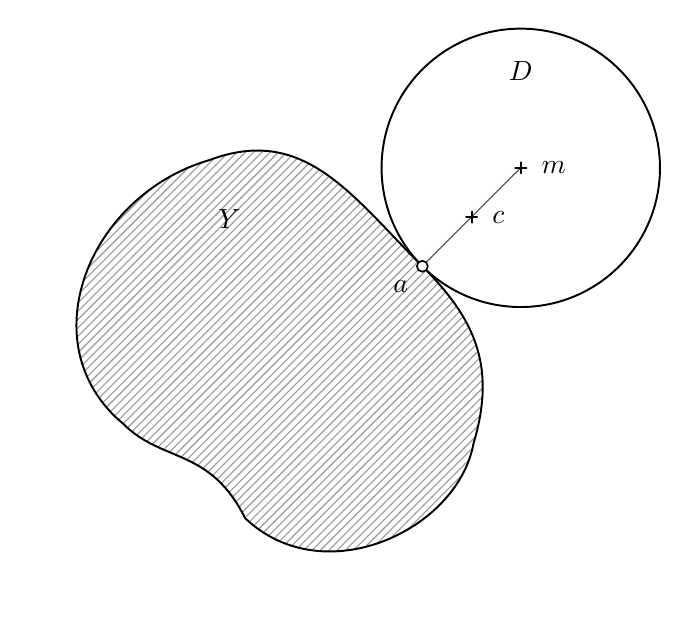
\begin{tikzpicture}[font=\normalsize]

\def\region{(0,0) .. controls (-.9,.9) and (-1.5,1.8) .. (-2.7,1.35) .. controls (-4.25,.9) and (-5,-1) .. (-3.8,-2) .. controls (-3.3,-2.5) and (-2.7,-2.3) .. (-2.25,-3.2) .. controls (-1.25,-4.15) and (.45,-3.35) .. (.65,-2.25) .. controls (.95,-1.25) and (.65,-.65) .. (0,0) -- cycle}
\fill[pattern=north east lines,pattern color=black!40] \region;
\draw[outline] \region;
\draw[outline] (1.25,1.25) circle[radius=1.76777];
\node at (-2.45,.6) {$Y$};\node at (1.25,2.48) {$D$};
\draw[line width=.45pt,black!65] (0,0)--(1.25,1.25);
\node[point,label=below left:$a$] at (0,0) {};
\draw[outline] (.555,.625)--(.695,.625) (.625,.555)--(.625,.695);
\draw[outline] (1.18,1.25)--(1.32,1.25) (1.25,1.18)--(1.25,1.32);
\node[right=4pt] at (.625,.625) {$c$};\node[right=4pt] at (1.25,1.25) {$m$};

\end{tikzpicture}
\end{document}
